%% LyX 2.3.0 created this file.  For more info, see http://www.lyx.org/.
%% Do not edit unless you really know what you are doing.
\documentclass[a4paper,journal]{IEEEtran}
\usepackage[latin9]{inputenc}
\usepackage{float}
\usepackage{booktabs}
\usepackage{amsmath}
\usepackage{graphicx}
\usepackage[unicode=true]
 {hyperref}
\usepackage{breakurl}
\usepackage{todonotes}

\makeatletter

%%%%%%%%%%%%%%%%%%%%%%%%%%%%%% LyX specific LaTeX commands.
\special{papersize=\the\paperwidth,\the\paperheight}

%% Because html converters don't know tabularnewline
\providecommand{\tabularnewline}{\\}
\floatstyle{ruled}
\newfloat{algorithm}{tbp}{loa}
\providecommand{\algorithmname}{Algorithm}
\floatname{algorithm}{\protect\algorithmname}

%%%%%%%%%%%%%%%%%%%%%%%%%%%%%% Textclass specific LaTeX commands.
% protect \markboth against an old bug reintroduced in babel >= 3.8g
\let\oldforeign@language\foreign@language
\DeclareRobustCommand{\foreign@language}[1]{%
  \lowercase{\oldforeign@language{#1}}}

%%%%%%%%%%%%%%%%%%%%%%%%%%%%%% User specified LaTeX commands.
\usepackage{graphicx}
\usepackage{url}
\usepackage{float}

\usepackage{algorithm}
\usepackage[noend]{algpseudocode}
\usepackage{graphicx}
\usepackage{subcaption}


\usepackage{hyperref}       % hyperlinks
\usepackage{url}            % simple URL typesetting
\usepackage{booktabs}       % professional-quality tables
\usepackage{amsfonts}       % blackboard math symbols
\usepackage{nicefrac}       % compact symbols for 1/2, etc.
\usepackage{smartdiagram}

\usetikzlibrary{fit}
\usepackage{pgfplots}
\DeclareMathOperator*{\argmax}{arg\,max}
\DeclareMathOperator*{\argmin}{arg\,min}
\makeatother

\begin{document}

\title{Decision Making Under Uncertainty for Urban Driving}

\author{Philippe Weingertner, Arnaud Autef, Simon Le Cleac'h}

\markboth{AA228 - Final Paper}{ }
\maketitle
\begin{abstract}
In this work we examine the problem of Motion Planning for Autonomous
Driving - AD. We must plan in a stochastic environment with several sources
of uncertainties: imperfect sensors, occlusions, unpredictable behaviour of external agents. We focus on sensor
uncertainties and model the AD problem as a Partially Observable Markov
Decision Process - POMDP - with a discrete action space and continuous state and observation spaces. We propose improvements to a traditional \textit{online} algorithm used for such large POMDPs: the POMCP algorithm. The goal is to make our motion planner a \textit{safer} autonomous driver. Our proposed solutions include: a "safe" discretization of the observation space, importance sampling techniques and an \textit{offline} preprocessing of the state space to limit the planner's behaviour to "safe" actions. We implemented and tested our methods on two AD environments: a Custom Anti-Collision Test Environment - CACTE - and the Urban Driving Environment - UDE - from Stanford's Intelligent Systems Laboratory - SISL.
\end{abstract}


\section{Problem Statement}

We consider the problem of determining a sequence of optimal actions
for a Urban Driving Motion Planner. The autonomous driving pipeline
consists of  modules with distinct roles: a \textbf{sensors fusion and localization} module producing a probabilistic model of the environment's dynamic, a \textbf{decision making} module defining a driving policy and a \textbf{motion control} module defining commands for the actuators. The decision making module can be further subdivided into three modules:
\begin{enumerate}
    \item \textbf{Route planner}: to define a long term driving goal.
    \item \textbf{Behavioral planner}: to define a list of short term objectives, typically going from A to B with a mixture of \textit{efficiency} (time taken) \textit{comfort} (minimizing jerk) and \textit{safety} (avoiding collisions and keeping safety distances) objectives.
    \item \textbf{Motion planner}: to complete the motion tasks submitted by the behavioral planner.
\end{enumerate}
\begin{center}
\begin{figure}[H]
\begin{centering}
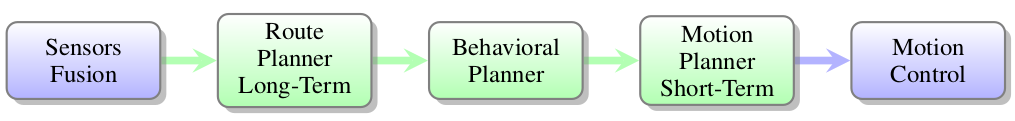
\includegraphics[width=9cm]{figures/pipeline.png}
\par\end{centering}
\centering{}\caption{Autonomous Driving Pipeline}
\label{fig:AD}
\end{figure}
\par\end{center}
We focus on the \textbf{Motion planner}, which can be thought as a module taking sequential decisions, in the form of a discrete set of actions (acceleration or deceleration) that will then be converted to a sequence of continuous actions by a command and control module (usually a simple Model Predictive Controller - MPC).\newline
The motion planner has to deal with several sources of uncertainties that are not directly observable: sensors uncertainties, occlusions and drivers intentions. Linking driving decisions to a proper handling of those sources of uncertainties is of paramount importance.\newline
In this paper we study how POMDP models can be applied to an
AD motion planner, and emphasize on the \textit{safety} objective of the Motion Planner: our proposed algorithm should succeed in their objective of going from position A to B with the strict requirement of avoiding any collision with other agents\newline
When dealing with huge states spaces, as it is the case in our urban driving setting, online methods are usually preferred over offline methods and our work starts from there. ``A Survey of Motion Planning and Control Techniques for Self-driving Urban Vehicles'' \cite{7490340}, reveals that most motion planning techniques somehow boil down to an online graph search. In the paper, we study how uncertainty can be properly modeled and handled during this online graph search process to improve safety, and also consider offline methods to guide this graph search and improve safety. 

\section{Related Work}

The \textit{Partially Observable Monte Carlo Planning} - POMCP - algorithm \cite{NIPS2010_4031} was proposed in 2010 to deal with large POMDPs, it is the starting point of our work. It was initially limited to discrete actions and observations space. In \cite{Bouton2017}, an AD task is solved using a
POMDP modeling of the environment along with an online POMCP solver. In order to deal with continuous state and continuous observation spaces a Progressive Widening technique was used. However, their work does not emphasize on safety in AD. A recent improvement to POMCP,  POMCPOW \cite{Sunberg2018} lets POMCP deal with continuous actions and observations.
The proposed method is strongly tied to particle filters within the search tree. According to its author, the particle filters inside of the tree could be customized, but it\textquoteright s not immediately
clear how to integrate a Kalman Filter. The Kalman Filter is the filter we decided to use because it is simple, fast and has
no particle deprivation issue. In \cite{Hoey:2005:SPC:1642293.1642505}
the idea of a lossless partitioning, with respect to the policy, of
the continuous observation space is introduced but the proposed approach
is limited to discrete states and relies on point-based backups (PBVI,
Perseus). The underlying idea is appealing to us and we decided to
explore how to take advantage of the structure of our problem to come
up with such a lossless partitioning of the continuous observation
space. In addition to POMCP, DESPOT is another online POMDP solver
that is providing state of the art results: it has been used in conjunction
with Importance Sampling in \cite{Luo2017ImportanceSF}. Dealing with
huge states spaces, as it is the case in urban autonomous driving,
online methods are usually preferred over offline methods. But using
an online method based on sparse sampling may lead to safety issues.
Rare events with critical consequences may not be sampled leading
to sub-optimal and potentially dangerous decisions. That is why using
Importance Sampling in conjunction with POMCP or DESPOT is important.
In addition to the sampling of observations, we bring another contribution to POMCP. We modify the action selection phase to add a safety criterion so that the car can only take actions that will not result in a collision, with a chosen level of confidence. This approach has been developed and tested in the AD setting in \cite{Bouton2018uai}. We use the same formulation for the offline computation of the safe actions, and we extend this approach to the POMDP setting, while \cite{Bouton2018uai} applied it to a fully observable MDP.
We build upon the work referred to previously and we will be using the
Julia POMDP framework from \cite{Egorov2017} for experimentation.

\section{Proposed Approach}

First, we describe the modelling of our two simulation environments by a POMDP 
\subsection{POMDP Models}
\subsubsection{Custom Anti-Collision test environment}
\textbf{State space} $\mathcal{S}$ and \textbf{observation} space $\mathcal{O}$ are continuous, they correspond to position and speed information for each car: 
\[
\{(x,y,v_{x},v_{y})_{ego},{(x,y,v_{x},v_{y})_{obj}}_{1..n}\}
\]
The \textbf{action space} $\mathcal{A}$ is discrete with $4$ actions corresponding to acceleration levels along a straight line:
\[
a \in\{-4\text{ }ms^{-2},-2\text{ }ms^{-2},0\text{ }ms^{-2},2\text{ }ms^{-2}\}
\]
The\textbf{ transition} and \textbf{observation} models are linear Gaussian with $Pr(P_{i}^{t+1}\mid P_{i}^{t})=\mathcal{N}(TP_{i}^{t},Q)$ and $Pr(O_{i}^{t}\mid P_{i}^{t})=\mathcal{N}(HO_{i}^{t},R)$. \newline
The \textbf{belief updater}  is a Kalman Filter.\newline
The \textbf{reward model} accounts for efficiency, comfort and safety objectives. Total reward is the sum of the following terms:
\begin{itemize}
    \item r\_efficiency $=a$ as we target full speed
    \item r\_comfort $=-1$ for hard breaking $a=-4\text{ }ms^{-2}$ $0$ otherwise
    \item r\_safety\_ttc $=(10-\text{smallest Time To Collision})*10$ if $ttc<10$
    \item r\_safety\_collision$=-1000$ in case of a collision
\end{itemize}

\subsubsection{Urban Driving Environment}
The UDE is a \textit{2D representation} of an AD task: the ego vehicle has to perform a left turn at a T-shaped intersection while avoiding two other cars driving on the main road. It is described in more details in part $IV$.\newline
The \textbf{state space} $\mathcal{S}$ includes, for each car:
\begin{itemize}
    \item The Cartesian coordinates of the car in the environment $x$, $y$, $\theta$. $\theta$ being the orientation of the car around its center.
    \item The Frenet coordinates of the car in the environment $s$, $t$, $\phi$, where $s$ and $t$ are the tangent and the normal coordinates of the car on its \textit{current} lane.
    \item The norm of the car's speed vector $v$.
    \item The dimensions ($width$, $length$) of the car.
    \item The car's \textit{driver model}, determining the car's driving behaviour (for the ego it is instead the motion planning algorithm selected).
\end{itemize}
The \textbf{action space} $\mathcal{A}$ is discretized and limited to $4$ actions.
The ego vehicule is following a \textit{predetermined} curve on the T-shaped intersection of the UDE, it is not allowed to drift from this curve and its actions are \textit{acceleration} levels of the vehicle along the curve at every time-step. The $4$ actions correspond to the following acceleration levels: 
\[
\{-4m/s^{-2},~-2m/s^{-2},~0m/s^{-2},~2m/s^{-2}\}
\]
The \textbf{observation space} $\mathcal{O}$ choice has been crucial, as we selected what our agent would be able to "see" during simulations. Observations are vectors of size $4 \times n_{cars}$. They are obtained by concatenating vectors $\left(d_{ego}, l, s, v\right)$ for each car, where $d_{ego}$ is the Euclidian distance (in meters) between the car and the ego vehicle, $l$ is the lane of the car, $s$ its tangent coordinate on the lane and $v$ its speed (in meters / second).\newline
The $state \rightarrow state'$ \textbf{transition} model is based on simple point mass dynamics. We added a \textit{transition noise} to transition dynamics of ($s$, $v$) for each car, in the form of a gaussian distribution with mean $0$ and variance $\sigma^2_{s} = 0.25 \:m^2, \sigma^2_{v} = 0.25 \:m^2.s^{-2}$.\newline
The $state \rightarrow observation$ \textbf{observation} model correspond to picking up the $\left(d_{ego}, l, s, v\right)$ values from the state and adding an \textit{observation noise} to ($s$, $v$), in the form of a gaussian distribution with mean $0$ and variance $\sigma^2_{s} = 1.0 \:m^2, \sigma^2_{v} = 1.0 \:m^2.s^{-2}$.\newline
The \textbf{belief updater}  is a Kalman Filter.\newline
The \textbf{reward model} if simple: a reward of $+1.0$ is granted when the agent reached the end of the intersection, any collision ends the simulation and yields a reward of $-1.0$. The discount factor for rewards is set at $\gamma = 0.95$.
\subsection{POMCP algorithm}
The POMCP algorithm \cite{NIPS2010_4031} is an extension of the traditional \textit{Monte Carlo Tree Search} algorithm to \textit{Partially Observable }Markov Decision Processes. In our attempt to solve the two POMDP models specified previously, we start from a variant of this algorithm, which maintains a \textit{belief b} in observation nodes of the search tree. The core of the algorithm is presented in Algorithm \ref{alg:pomcpsimple} and the rollout routine in Algorithm \ref{alg:pomcpsimplerollout}.
\begin{algorithm}[h]
\begin{algorithmic}[1] 
\Function{SelectAction}{$b,d$} 
	\State $h \gets \emptyset$
	\Loop
		\State \Call {Simulate}{$b,h,d$}
	\EndLoop
	\State \Return arg max$_a\text{ }Q(h,a)$
\EndFunction

\Function{Simulate}{$b, h,d$} 
	\If {$d=0$}
		\State \Return $0$
	\EndIf



	\State $a \gets \text{arg max}_a\text{ }Q(h,a)+c\sqrt{\frac{logN(h)}{N(h,a)}}$
	\State $s \sim b$
	\State $(s',o,r) \sim G(s,a)$

	\If {$hao \notin T$}
		\For {$a \in A(s)$}
			\State $(N(h,a),Q(h,a)) \gets (N_0(h,a),Q_0(h,a))$
		\EndFor

		\State $T=T \cup \{hao\}$
		\State \Return \Call {Rollout}{$b,d,\pi_0$}
	\EndIf
	\State $b' \gets \Call {UpdateBelief}{\text{b,a,o}}$
	\State $q \gets r+\lambda$ \Call {Simulate}{$b',hao,d-1$}
	\State $N(h) \gets N(h)+1$
	\State $N(h,a) \gets N(h,a)+1$
	\State $Q(h,a) \gets Q(h,a)+ \frac{q-Q(h,a)}{N(h,a)}$
	\State \Return $q$ 
\EndFunction
\end{algorithmic}
\caption{POMCP algorithm}
\label{alg:pomcpsimple}
\end{algorithm}

\begin{algorithm}[h]
\begin{algorithmic}[1] 
\Function{Rollout}{$b,d,\pi_0$} 
	\If {$d=0$}
		\State \Return $0$
	\EndIf
	\State $a \sim \pi_0(b)$
	\State $s \sim b$
	\State $(s',o,r) \sim G(s,a)$
	\State $b' \gets \Call {UpdateBelief}{\text{b,a,o}}$
	\State \Return $r+\lambda$ \Call {Rollout}{$b',d-1,\pi_0$}
\EndFunction

\end{algorithmic}

\caption{Rollout evaluation}
\label{alg:pomcpsimplerollout}
\end{algorithm}

\subsection{Safe variants of POMCP}
Then, we make some modifications to this basic POMCP algorithm to improve performances of our policies in terms of safety, where safety corresponds to the collision rate of our ego vehicle with other agents and should be as close as possible to $0$.

\subsubsection{Safe discretization of observations}
In the CACTE and UDE, the observation space is \textit{continuous}, and very hard to discretize. In CACTE for instance, when considering a scene with 10 objects, observations are vectors of 40 real coordinates. Therefore, With POMCP, for every tree query, a previously unseen observation will be sampled. If this observation does not belong
to the tree, a new node will added. By using POMCP with continuous
observations, the probability of sampling identical observations is
zero, and the end result is a shallow tree, see figure \ref{fig:shallow_and_deep_trees}. Technically POMCP will execute without error but will return a significantly sub-optimal solution. 

After considering potential use of POMCP with DPW or POMCPOW to deal
with continuous observations, we developed our own POMCP variant
by taking advantage of the structure of our AD problem.
Ideally we would like to be able to limit the number of observation
nodes in the tree so that we can explore the tree in depth and keep
the capability to do belief updates during the rollout evaluation with continuous observations.

When aggregating observations, we would like grouped observations to correspond to similar utilities. The utility function is highly safety-dependent. In the CACTE, it also depends on efficiency and comfort, but both are action rather than observation dependent. Therefore, grouping together observations according a safety criteria looked reasonable, and a good way to improve safety, let us describe the procedure with both environments:
\begin{itemize}
    \item In \textbf{CACTE}, for every single observation, we evaluate the smallest Time To Collision to the 10 objects observed and create 11 observations classes corresponding to a TTC ranging from less than 1, to less than 10, with any other smallest TTC value above 10 being aggregated into the lowest collision risk category. We create observations classes that should correspond to same safety utility or a somewhat more pessimistic safety value.
    \item In the \textbf{UDE}, we create classes of observations based on the distance between the ego car and the closest car in the scene. We define 20 observations classes corresponding to distances between 0 and 10 meters (the last class containing all distances above 10m). 
\end{itemize}

 

\begin{center}
\begin{figure}[H]
\begin{centering}
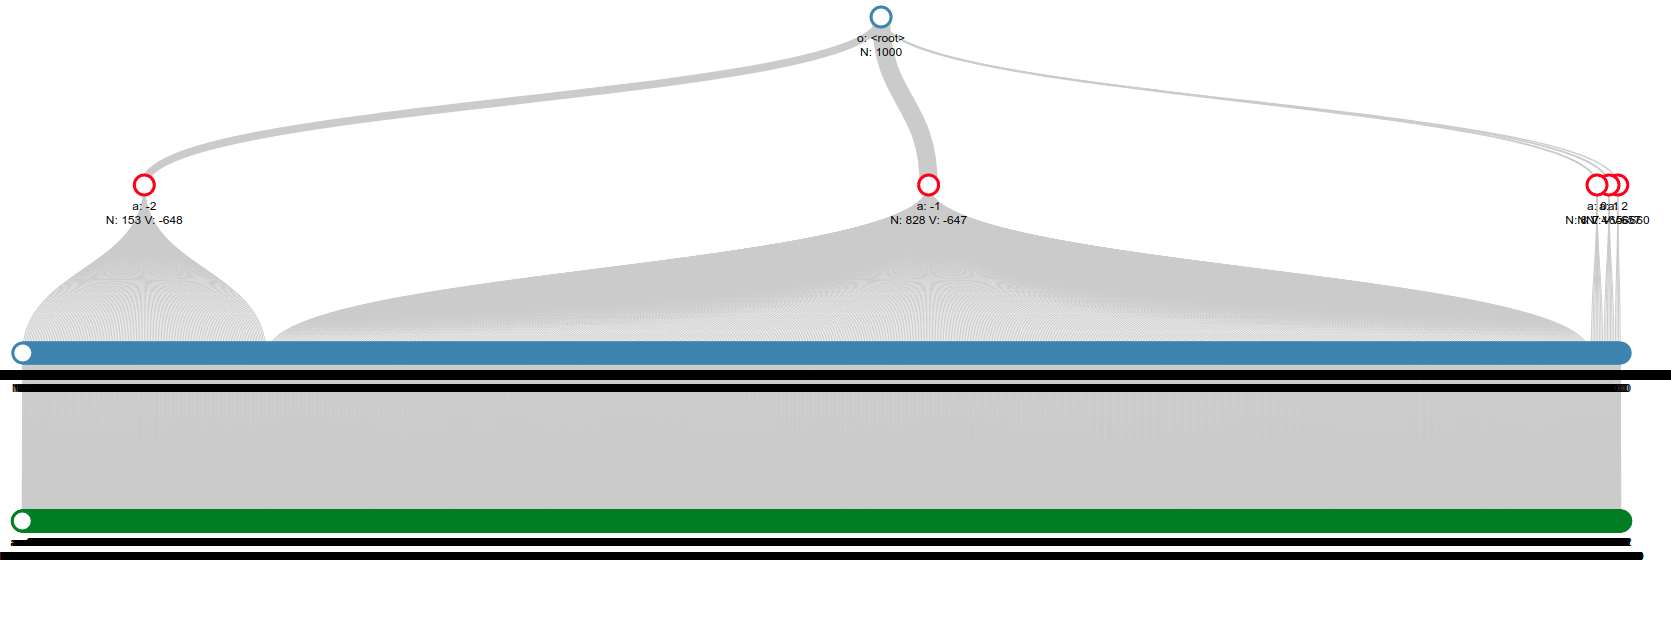
\includegraphics[scale=0.07]{figures/BasicPOMCP}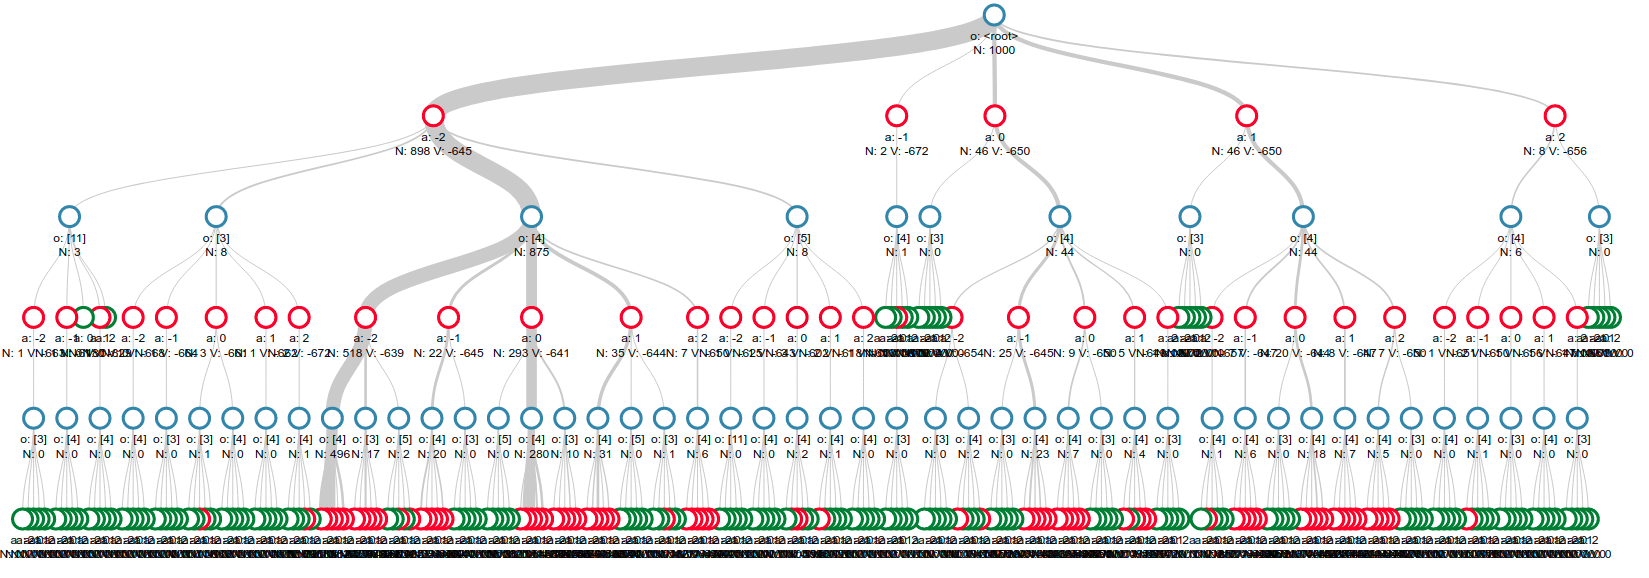
\includegraphics[scale=0.07]{figures/BasicPOMCPTtc1TreeSearch}
\par\end{centering}
\centering{}\caption{With safe clusterization of observations (right)}
\label{fig:shallow_and_deep_trees}
\end{figure}
\par\end{center}

In both settings, for every observation class node, we keep track of the most recent raw observation. This raw observation value is used to update the belief node with a Kalman Filter.

While this solution is taking advantage of the structure of our problem
it highlights some more general ideas that could be re-used to apply
POMCP algorithm to problem with continuous observations:
\begin{itemize}
\item Observations nodes are aggregated per Utility class
\item We have a dual capability to use a discretized version of the observation
when handling MCTS tree expansion while still using a continuous observation
for BeliefUpdate in a way that would be adapted to elaborate Importance Sampling
approach, where we want to prioritize the sampling of collision scenarios in the tree to efficiently avoid them.
\end{itemize}
The proposed modification of POMCP algorithm is presented in Algorithm \ref{alg:modifiedpomcp} and Algorithm \ref{alg:modifiedpomcpclusterizing}.
\begin{algorithm}[h]
\begin{algorithmic}[1] 
\Function{SelectAction}{$b,d$} 
	\State $h \gets \emptyset$
	\Loop
		\State \Call {Simulate}{$b,h,d$}
	\EndLoop
	\State \Return arg max$_a\text{ }Q(h,a)$
\EndFunction

\Function{Simulate}{$b,h,d$} 
	\If {$d=0$}
		\State \Return $0$
	\EndIf



	\State $a \gets \text{arg max}_a\text{ }Q(h,a)+c\sqrt{\frac{logN(h)}{N(h,a)}}$
	\State $s \sim b$
	\State $(s',o,r) \sim G(s,a)$
	
	\State $o_{class}, ttc \gets \Call {ClusterizeObservation}{\text{s',o}}$

	\If {$hao_{class} \notin T$}
		\For {$a \in A(s)$}
			\State $(N(h,a),Q(h,a)) \gets (N_0(h,a),Q_0(h,a))$
		\EndFor
		
		\State $o_{class}^{id}  = o_{class}, o_{class}^{ttc} = ttc, o_{class}^{raw} = o$

		\State $T=T \cup \{hao_{class}\}$
		\State \Return \Call {Rollout}{$b,d,\pi_0$}
	\ElsIf {ttc $< o_{class}^{ttc}$}
		\State $o_{class}^{ttc} = ttc, o_{class}^{raw} = o$
	\EndIf
	\State $b' \gets \Call {KalmanUpdater}{\text{b,a,o}}$
	\State $q \gets r+\lambda$ \Call {Simulate}{$b',hao_{class},d-1$}
	\State $N(h) \gets N(h)+1$
	\State $N(h,a) \gets N(h,a)+1$
	\State $Q(h,a) \gets Q(h,a)+ \frac{q-Q(h,a)}{N(h,a)}$
	\State \Return $q$ 
\EndFunction
\end{algorithmic}

\caption{Modified POMCP Tree Search}
\label{alg:modifiedpomcp}
\end{algorithm}

\begin{algorithm}[h]
\begin{algorithmic}[1] 
\Function{ClusterizeObservation}{$s', o$} 
	\State $ttc \gets \Call {SmallestTimeToCollision}{$s',o$}$
	\State $o_{class} = floor(min(ttc, 11))$
	
	\State \Return $o_{class}, ttc$
\EndFunction

\end{algorithmic}

\caption{Clusterize observation}
\label{alg:modifiedpomcpclusterizing}
\end{algorithm}

For rollout evaluation we keep on using continuous observations to
update our belief with a Kalman Filter and we sample continuous states.
The discretization of observations was used only during the tree expansion
phase: to limit the tree width extension so that we can explore the
tree in depth.



\subsubsection{Reward shaping}

The base reward used to guide our policies is a sparse reward where we get a large penalty in case of collision. To improve safety, we propose to shape this reward according to safety metrics. In the CACTE, reward shaping takes the form of reward that is proportional to the smallest computed Time To Collision w.r.t. any other cars detected. In the UDE, we explore increased reward penalties for collisions.

\subsubsection{Safe exploration with constrained actions}
\label{sec:value_iteration_section} %this label is used in Experimental setup
The last technique we propose to enforce safety is to adapt the work of Bouton and al. in \cite{Bouton2018uai} to the partially observable setting. In their work, they propose an interesting offline method to ensure safety in an AD setting, they use a fully observable model of the AD task, discretize the state space, and apply a \textit{Value Iteration} algorithm to compute:
\[
\mathbb{P}_{collision}(s, a),~\forall s, a \in \mathcal{S} \times \mathcal{A}
\]
Where those collision probabilities are obtained performing "safe Bellman updates" until convergence:
\[
\mathbb{P}^{k+1}_{collision}(s,a) = \sum_{s'}T(s'|s, a)\min_{a'}\mathbb{P}^{k+1}_{collision}(s',a')
\]
$\forall s, a \in \mathcal{S} \times \mathcal{A}$, with $\mathbb{P}_{collision}(s) = 1$ for collision states, $\mathbb{P}_{collision}(s) = 0$ for terminal and non-colliding states, $\mathbb{P}_{collision}(s)$ initialized to $0$ for other states. Then, a threshold for safety $0< t <1$ is selected, and the AD car is restricted in the actions $a$ it can take by the condition $\mathbb{P}_{collision}(s, a) < 1 - t$. For instance, with a safety level $t=0.999$, $\mathbb{P}_{collision}$ must be below $0.1\%$. If $\min_a \mathbb{P}_{collision}(s, a) \ge 1 - t$, agent must select $a^*(s) = \argmin_a \mathbb{P}_{collision}(s, a)$ \newline
In our work, we adapted this work to the \textit{Partially Observable} setting, where we work with \textit{beliefs b} rather than states. Our approach is the following:
\begin{enumerate}
    \item Compute the same offline safety preprocessing on a discretized version of $\mathcal{S}$ and get $\mathbb{P}_{collision}(s, a),~\forall s, a \in \mathcal{S} \times \mathcal{A}$
    \item Set a safety threshold $t$
    \item When agent is in belief $b$, make the approximation:
    \[
    \mathbb{P}_{collision}(b, a) \approx \int_{s}b(s)\mathbb{P}_{collision}(s, a)ds
    \]
\end{enumerate}
This approach allowed us to transfer this safety improvement technique to the partially observable setting, and interesting remarks can be made:
\begin{itemize}
    \item The approximation above is similar to the one made with the \textbf{QMDP} approach to POMDPs: for the approximation to be valid, the environment should fully observable after an intial sampling from the belief $b$.
    \item We have $two$ external cars in our environment, which would have made value iteration two expensive on a discretized version of the state space with two cars. We solve value iteration on a state space with a single external car, and take the following \textbf{utility decomposition} approach:
    \[
    Act(b) = Act(b)_{first\_car} \cap Act(b)_{second\_car}
    \]
    Where $Act(b)_{car}$ is the set of available actions using our above approximation when looking at potential collisions only with this car. If $Act(b) = \emptyset$, we compute $\min_a \mathbb{P}_{collision}(b_{car}, a)$ for the two cars, take the maximum (i.e look at the\textbf{ most dangerous} car), and select the according \textbf{safest} action $\argmin_a \mathbb{P}_{collision}(b_{car}, a)$.
\end{itemize}


\subsection{Other possible approaches}

\paragraph{Exhaustive online forward search}
We also consider what it would take to perform an exhaustive online
forward search. By using the observation discretization scheme proposed
previously, the complexity of an exhaustive online Forward Search
would be: $O(|A|^{d}|O|^{d}).$With $|A|=5$ and $|O|$ being reduced
to 10, we would be able to consider a forward search up to a depth
of 5. With a time step of 250 ms, this corresponds to a $1.250$ seconds
horizon.
\paragraph{Exact solution with Linear Gaussian dynamics and quadratic reward}
One very interesting point to consider here, is that we have a linear-Gaussian
dynamics model: $T(z\mid s,a)=\mathcal{N}(z\mid T_{s}s+T_{a}a,\Sigma)$.
As long as we consider a state vector of the form $s=[x,y,v_{x},v_{y}]$
and a discrete action that corresponds to an acceleration or deceleration
command this condition is fulfilled. If we could express the reward
function with a quadratic form, then it can be shown that the optimal
policy can be computed exactly offline. We refer to the ``Decision
Making under Uncertainty'' book in \cite{Kochenderfer2015} sections
6.4.6 and 6.2.2 for more details. The reward should be expressed in
a form $R(s,a)=s^{T}R_{s}s+a^{T}R_{a}a$ where $R_{s}=R_{s}^{T}\leq0,R_{a}=R_{a}^{T}<0$.
This is a very interesting property that we should take advantage
of. This would require further investigations.

\section{Experimental Setup}

\subsection{Custom Anti-Collision Test Environment}

While the SISL Urban Driving environment is great, building the CACTE was a good way to learn and better understand
some details in the process of using and interfacing the juliaPOMDP
framework. This environment is useful for tests in unstructured environments without lanes and roads constraining the
traffic of other cars, see figure \ref{fig:act_env}.

This environment can be downloaded from:  \href{https://github.com/PhilippeW83440/ACT}{Anti-collision Tests Link}.
It depends on a very limited number of packages and allows to experiment
with a complex high dimensional POMDP with 1 egovehicle and 10 moving
objects in the scene (more can be easily added). It enables to benchmark
performances both in terms of runtime and various performance metrics: efficiency,
comfort and safety. It is lightweight tool to create challenging anti-collision
tasks.

\begin{figure}[h]
    \centering
    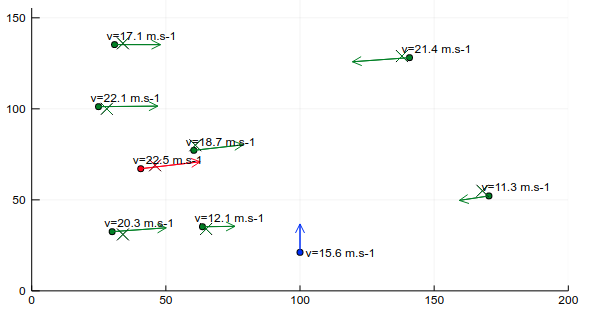
\includegraphics[width=0.48\textwidth]{figures/act_env.png}
    \caption{The anti-collision test environment, the ego car (blue dot) has to avoid 10 other vehicles (red and green dots).}
    \label{fig:act_env}
\end{figure}

\subsection{SISL Urban Driving environment}

To evaluate our safe variants of POMCP, we rely on the SISL Urban Driving environment that is used in \cite{Bouton2018uai}. We focus on the intersection setting shown in figure \ref{fig:intersection}. In this environment there are always two cars in the scene in addition to the ego car. The ego car has to make a left turn to reach the goal while avoiding any collision. All three cars are following a predetermined route and always stays in the middle of their lanes. For the ego car, we are controlling the acceleration $a$ of the vehicle along the predefined trajectory. We restrict our action space $\mathcal{A}$ to $a \in [-4, -2, 0, 2]$. The two other cars follow a rule-based policy: they give the priority to other vehicles when turning left and use the time to collision to make a crossing decision. Otherwise they are following the Intelligent Driver Model \cite{treiber}. In this environment, we test the POMCP algorithm with observation clustering and action selection safety criterion (Safe RL). For comparison we also test the version without the action selection safety criterion (Regular RL).

To apply Safe RL, we discretize the state space containing all the possible configurations of the ego car and another car in the scene. We discretize the longitudinal velocities of both cars and their positions along the lanes present in the scene. We obtain a discretized state space of 330.000 states and apply the value iteration algorithm described in \ref{sec:value_iteration_section} to get the safety criterion. We set the safety threshold to $t = 0.9999$. 

\begin{figure}[h]
    \centering
    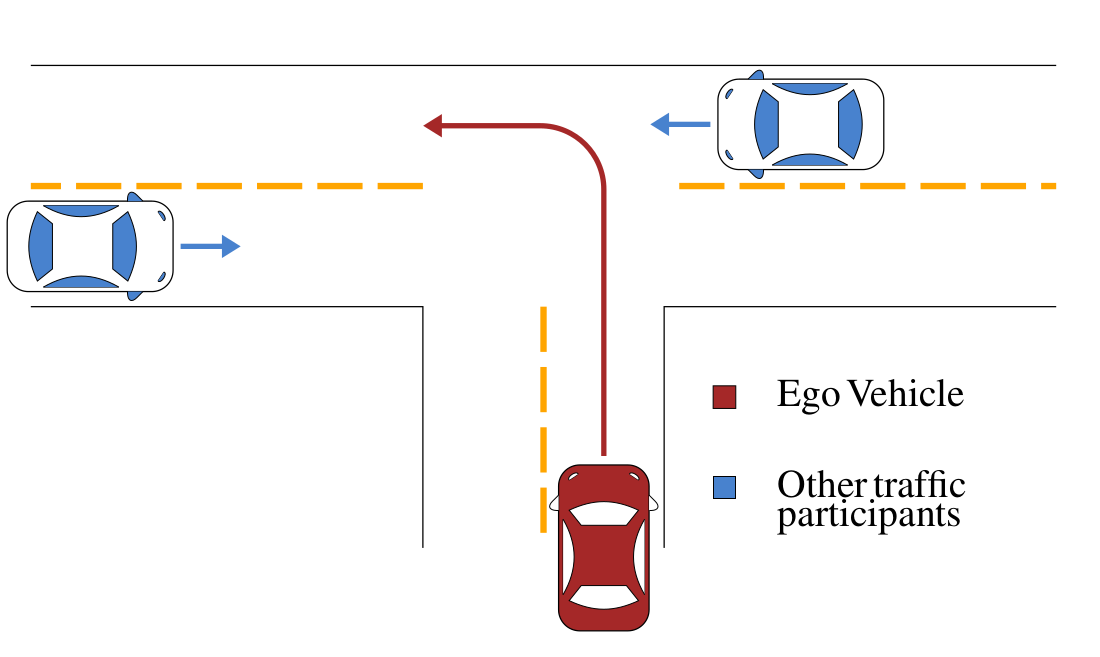
\includegraphics[width=0.48\textwidth]{figures/intersection_sketch.png}
    \caption{The ego vehicle have to perform a left turn at an unsignalized intersection while avoiding the other vehicles. Figure taken from \cite{Bouton2018uai}.}
    \label{fig:intersection}
\end{figure}

\section{Results}

\subsection{Results on the Custom Anti-Collision Test Environment}

\subsubsection{Processing time and exploration depth results}

In the below tests, the max\_depth is set to 20. The tree\_queries
parameter is increased and we check the maximum exploration depth
i.e. how deep we can explore and exploit the search tree. We use a
time step of 200 ms in our Transition Model. So an exploration depth
of 10 corresponds to an exploration up to a 2 seconds time horizon.

As a reminder without our POMCP modification, as observations are continuous,
the exploration depth is 1. 

Results have been obtained on a 7th generation intel core i7 processor, without any
specific optimization or multithreading.

\begin{table}[H]
\caption{POMCP results}

\centering{}%
\begin{tabular}{ccc}
\toprule 
tree\_queries & runtime & max exploration depth\tabularnewline
\midrule
\midrule 
100 & 35 ms & 5\tabularnewline
\midrule 
500 & 160 ms & 10\tabularnewline
\midrule 
1000 & 320 ms & 12\tabularnewline
\midrule 
2000 & 640 ms & 14\tabularnewline
\bottomrule
\end{tabular}
\end{table}


\subsubsection{Accuracy results}

The scenario is quite challenging and default policies generally
fail. The \textit{Time To Goal} and \textit{Number of hard breaking decisions} performance metrics are averaged over the scenarios that did not result in a collision.

We run exactly the same set of tests with the different policies.
\begin{itemize}
\item policy\_v0 is the default one (pomcp legacy and sparse reward).
\item policy\_v1 is based on pure predicted time to collision. This is our
real baseline. Not making use of the POMDP model.
\item policy\_v2 is based on reward reshaping based on time to collision
with legacy POMCP (pomcp legacy + reshaped reward)
\item policy\_v3 is with the modified pomcp. It is the policy that is POMDP
based (with exploration depth \textgreater{} 1) with a modified POMCP.
\end{itemize}
Policy\_v1 and policy\_v2 yield exactly the same results, which is expected as using POMCP with policy\_v2 does not give improvements: observations are continuous and we do not explore the tree at all.

\begin{table}[H]
\caption{Benchmark results}

\centering{}%
\begin{tabular}{cccc}
\toprule 
 & \% Collisions & Time To Goal & Hard Breaking\tabularnewline
\midrule
\midrule 
policy\_v0 & 80\% & 11 s & 8\tabularnewline
\midrule 
Baseline policy\_v1 & 60\% & 11.8 s & 10\tabularnewline
\midrule 
policy\_v2 & 60\% & 11.8 s & 10\tabularnewline
\midrule 
policy\_v3  & 0\% & 12.8 s & 10\tabularnewline
\bottomrule
\end{tabular}
\end{table}

As expected, we get clearly better safety results with policy\_v3. 

\subsection{Results on SISL Urban Driving environment}

\subsubsection{Offline Computation of the safe actions}

To determine the set of safe actions for a given a belief, we compute the value iteration described in \ref{sec:value_iteration_section} with a discretized state space of size 330.000. This value iteration takes 2 hours to run on a i-core7 platform without any specific optimization or multithreading. At the end of the optimization, we get a Bellman Residual of $10^{-5}$. Which means that our computation of $\mathbb{P}_{collision}(s,a)$ through value iteration is precise up to the fourth digits. This is consistent with the threshold value that we selected to ensure safety: $t = 0.9999$. We visualize in figure \ref{fig:histogram} the repartition of the tuples of discretized states and actions $(s,a)$ according to their safeties defined by $\mathbb{P}_{collision}(s,a)$. 

\begin{figure}[h]
    \centering
    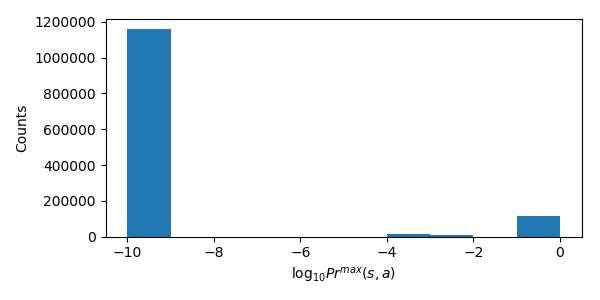
\includegraphics[width=0.48\textwidth]{figures/histogramModelChecking.png}
    \caption{Histogram presenting the repartition of the state-action pairs $(s,a)$ according to their safety values. The safest states are on the left of the chart.}
    \label{fig:histogram}
\end{figure}
 
\subsubsection{Exploration with constrained actions}
This problem has two conflicting objectives: efficiency which we define as the time required to reach the objective, and safety. We compare the Regular RL and Safe RL algorithms for different reward settings.  We vary the collision cost between 0.5 and 8 for both solution methods and estimate their performance. The performance is defined by computing the mean number of timesteps needed to reach the goal (efficiency criterion) and the collision rate (safety criterion). We perform 20 rollouts of each algorithm for each value of the collision cost. The tree exploration is parameterized by the number of tree queries of 100 at each time step, ad the exploration parameter $c = 0.1$. Based on these simulations, we draw the Pareto frontiers shown in figure \ref{fig:pareto_curve}. 

On this chart the optimal region is in the bottom-left corner. We can see that Regular RL can reach points that are more efficient than those obtained with Safe RL. However, the chart shows that Safe RL can outperform Regular RL on the safety criteria while having an efficient policy. This indicates that the Safe RL algorithm can generate policies with performances that could not be reached by applying reward shaping to Regular RL. 


\begin{figure}[h]
    \centering
    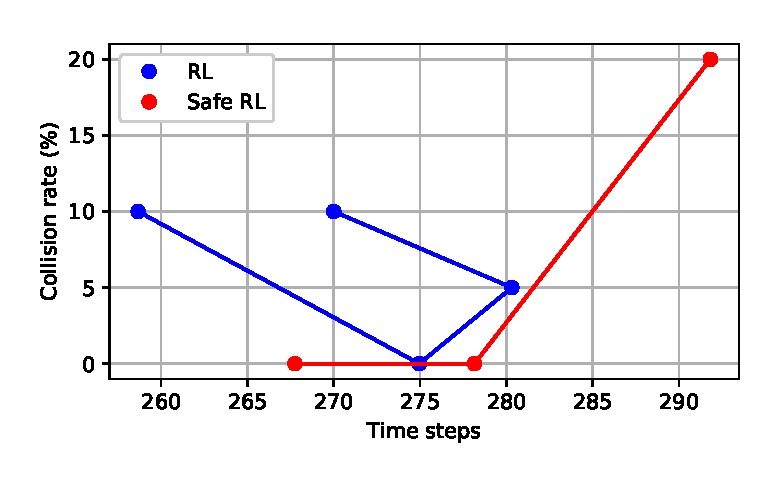
\includegraphics[width=0.48\textwidth]{figures/pareto_curve_v0_v1_vectorized.eps}
    \caption{Pareto frontiers obtained using the Safe RL and regular RL algorithms. These frontiers corresponds to different behaviors in terms of safety and efficiency induced by variations in the collision cost in the reward function.}
    \label{fig:pareto_curve}
\end{figure}
 


\section{Conclusion}

We came up with a detailed POMDP formulation of the problem of Motion
Planning for an Autonomous Driving car dealing with sensors uncertainty and proposed several improvements to the legacy POMCP solver to enforce safety. We handled the issue of continuous observations in a high dimensional POMDP and proposed several safety improvement techniques. We provided reference implementations and benchmark results on a set of tests to validate the proposed ideas. Further work could involve:
\begin{itemize}
    \item The ego vehicle is currently constrained to longitudinal accelarations on a curve, we could explore more complex 2d scenarios, and include pedestrians in the environment.
    \item Using value iteration on a discretized \textit{belief} rather than \textit{state} space to compute the safe actions. It would improve safety and let us avoid a "QMDP-like" assumption. Belief space discretization could be driven by safety criteria, in the same line than our modification of POMCP to handle continuous observations.
    \item Pure offline methods similar to the ones used for aircraft collision avoidance
    \cite{6301081} could be considered as well.
    \item Finally, it would be interesting to explore \textit{online} safety methods to constrain actions compared to an \textit{offline} preprocessing of the discretized state space.
\end{itemize}  

\bibliographystyle{plain}
\nocite{*}
\bibliography{bibliography}


\appendices{}
\end{document}
